\documentclass[conference]{IEEEtran}
\usepackage[utf8]{inputenc}
\usepackage[T1]{fontenc}
\usepackage{graphicx}
\usepackage{booktabs}
\usepackage{array}
\usepackage{listings}
\usepackage{xcolor}
\usepackage{tikz}
\usetikzlibrary{positioning,arrows.meta,fit}
\usepackage{cite}
\usepackage[hidelinks]{hyperref}

\lstset{basicstyle=\ttfamily\footnotesize,columns=fullflexible,breaklines=true,
  frame=single,framerule=0.3pt,xleftmargin=2pt,xrightmargin=2pt,aboveskip=4pt,belowskip=4pt}
\newcommand{\code}[1]{\texttt{#1}}

\begin{document}

\title{AutoGrader: A Rule-Driven Agent for\\Grading C Programs}

\author{
\IEEEauthorblockN{Shakti Prasad Nahak (2611AI46), Akash Prasad (2611AI08),\\
Gourav Rajak (2611AI07), Bibaswan Das (2611MC16)}
\IEEEauthorblockA{Department of Computer Science and Engineering, IIT Patna\\
CS5103 Agentic AI Lab, Course In-charge: Prof.\ Arijit Mondal}
}

\maketitle

\begin{abstract}
Checking a class's C programs by hand is slow, and two TAs rarely give the same mark for the
same mistake. We built AutoGrader, an agent that takes a student's \code{.c} file and an
instructor's \code{rules.json}, runs the program inside a locked Docker container, scores it
with one analyzer per metric, and returns a single grade with feedback. When the program is
wrong, the report shows the input that breaks it, the expected output and what the program
printed. Copying is detected with winnowed fingerprints and an AST comparison against
classmates, saved web solutions, solutions generated by a local LLM, and the instructor's own
solution. The LLM (Qwen2.5-Coder 7B through Ollama) runs on the same machine and only scores
readability and writes advice; it never decides correctness. On the 15 sample submissions the
grades are identical across repeated runs, and all 928 automated tests pass, including 14
deliberately malicious programs.
\end{abstract}

\begin{IEEEkeywords}
automated grading, program analysis, sandboxing, plagiarism detection, LLM agents
\end{IEEEkeywords}

\section{Introduction}
A programming lab with 60 students and one assignment a week produces about 60 programs to
compile, run, read and mark every week. Most of that time goes into the same steps: compile,
feed some inputs, compare the output, look at the code. The steps are mechanical, but the
marks are not consistent when different people do them, and copied solutions are easy to miss
when nobody compares all pairs.

The assignment asked for an agent that does the whole job without a person in the loop and
gives the same grade every time it sees the same file under the same rules. We split the work
into small analyzers that each judge one thing (correctness, warnings, structure, memory
safety and so on) and a coordinator that decides which analyzers can run, runs them, and adds
up their scores using the weights in the rules file.

Section~\ref{sec:req} lists the requirements and where each one is met.
Section~\ref{sec:design} describes the design, Section~\ref{sec:eval} reports the results on
the sample submissions and our tests, and Sections~\ref{sec:use} and~\ref{sec:lim} give the
usefulness and the limitations the assignment asks for.

\section{Requirements}\label{sec:req}
Table~\ref{tab:req} maps the six requirements of the assignment to the part of the system that
handles them.

\begin{table}[!t]
\caption{Assignment requirements and where they are met}\label{tab:req}
\centering\footnotesize
\begin{tabular}{@{}>{\raggedright\arraybackslash}p{0.36\columnwidth}>{\raggedright\arraybackslash}p{0.56\columnwidth}@{}}
\toprule
Requirement & Implementation \\
\midrule
R1 Run safely with time and memory limits & Docker container per job: no network, read-only root, all capabilities dropped, 64 processes, memory cap, \code{timeout} and \code{prlimit} per run \\
R2 Rules outside the code & \code{rules.json} per problem: metric, analyzer, weight, parameters; checked on load \\
R3 One analyzer per metric & 11 analyzers behind one interface; the coordinator runs them in parallel \\
R4 Unattended, reproducible & CLI and web app; fixed seeds, instruction counts instead of timings, cached LLM replies \\
R5 Failing input with expected output & hidden tests, named edge cases and 100 seeded random trials, all checked against the reference solution; failing inputs are shrunk \\
R6 Usefulness and limitations & Sections~\ref{sec:use} and~\ref{sec:lim}, and a short block in every report \\
\bottomrule
\end{tabular}
\end{table}

\section{Design}\label{sec:design}

\subsection{Overview}
Fig.~\ref{fig:arch} shows the parts. A student uploads a file through the React web page or
the instructor runs the command line tool. The FastAPI server never runs student code: it
stores the file and adds a job to a table in SQLite. A separate worker process claims the job,
starts a sandbox, and calls the coordinator. The worker sends a heartbeat while it works, and
a reaper puts the job back in the queue if a worker dies. Progress is streamed to the browser
with server-sent events.

\begin{figure}[!t]
\centering
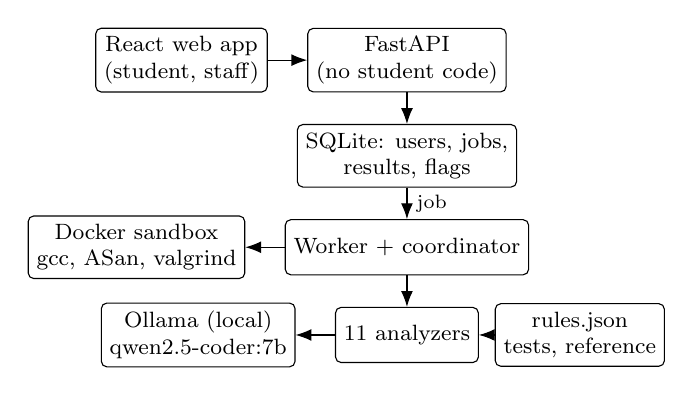
\begin{tikzpicture}[font=\footnotesize, node distance=4mm and 5mm,
  box/.style={draw, rounded corners=2pt, align=center, minimum height=7mm, inner sep=3pt},
  arr/.style={-{Latex[length=2mm]}}]
\node[box] (ui) {React web app\\(student, staff)};
\node[box, right=of ui] (api) {FastAPI\\(no student code)};
\node[box, below=of api] (db) {SQLite: users, jobs,\\results, flags};
\node[box, below=of db] (wk) {Worker + coordinator};
\node[box, left=of wk] (sb) {Docker sandbox\\gcc, ASan, valgrind};
\node[box, below=of wk] (an) {11 analyzers};
\node[box, left=of an] (llm) {Ollama (local)\\qwen2.5-coder:7b};
\node[box, right=of an, xshift=-3mm] (rules) {rules.json\\tests, reference};
\draw[arr] (ui) -- (api);
\draw[arr] (api) -- (db);
\draw[arr] (db) -- node[right]{\scriptsize job} (wk);
\draw[arr] (wk) -- (sb);
\draw[arr] (wk) -- (an);
\draw[arr] (an) -- (llm);
\draw[arr] (rules) -- (an);
\end{tikzpicture}
\caption{Components. Only the worker touches student code, and only inside the sandbox.}
\label{fig:arch}
\end{figure}

\subsection{Rules file}
Each problem has a folder with \code{rules.json}, the reference solution, a sample input, the
hidden tests and an optional corpus of known solutions. The rules list the metrics. Each metric
names its analyzer, a weight, and parameters for that analyzer:

\begin{lstlisting}
{ "name": "logical",
  "analyzer": "edge_case_runner",
  "weight": 0.10,
  "params": {
    "cases": ["negatives", "zero", "int_overflow"],
    "random_trials": 100,
    "seed": 7 } }
\end{lstlisting}

On load the rules are validated: the weights must add up to 1.0, every analyzer must exist,
sizes and limits must be positive. An error is reported with the field that caused it, before
any student is graded. Changing a weight or a threshold only needs an edit to this file. The
SHA-256 of the canonical rules is stored in every report, so a grade can always be traced to
the exact rules that produced it.

\subsection{Sandbox}
Every grading job gets a new Docker~\cite{merkel2014} container from our image \code{autograder-sandbox:1} (Debian,
gcc~12, valgrind~3.19, cppcheck~2.10). It runs with \code{-{}-network none},
\code{-{}-read-only}, \code{-{}-cap-drop ALL}, \code{no-new-privileges}, a limit of 64 processes,
one CPU and a memory cap. Each run of the student binary is further wrapped in \code{timeout}
and \code{prlimit} with the limits from the rules (1~s and 64~MB in our examples), and its
output is cut off after a fixed size. The reference solution is compiled and run in a second
container, so a submission cannot overwrite or replace the reference binary. We added this
after finding that a submission which deleted and rewrote the reference in a shared container
could make the comparison agree with its own wrong output.

\subsection{Coordinator}
The coordinator works in four steps.

\emph{First pass.} It compiles with \code{gcc -O2 -Wall -Wextra -std=c11}, runs the sample
input under the time and memory limits, and checks that \code{main}, an input call and an output
call exist. It also scans the tokens (with comments removed) for calls such as \code{system},
\code{fork} and \code{socket} and records them as flags.

\emph{Plan.} If the program does not compile, the analyzers that need a binary are skipped and
the quality metrics get no marks, because a program that cannot be built should not collect
points for neat style. If the sample run times out, the report gets the
\code{suspected\_infinite\_loop} flag, the run-based analyzers are skipped, and the source-only
analyzers still run. The report is then marked as partial.

\emph{Dispatch.} The analyzers run in parallel. Each one gets the source, the binary, the
sandbox and only its own parameters, and returns a score between 0 and 1, its evidence, and a
feedback line. An analyzer that crashes gets 0 and an error note; it does not stop the others.

\emph{Combine.} The grade is $\sum_i s_i w_i \times 100$, rounded to one decimal. A metric marked
``review only'' gives no points, and the remaining weights are scaled back up to 100. If the
program passes none of the hidden tests, the complexity metric is not credited, because a fast
program that prints the wrong answer is not efficient.

\subsection{Analyzers}
Table~\ref{tab:an} lists the analyzers. Akash Prasad wrote the execution analyzers, Gourav Rajak
the code-quality analyzers, and Bibaswan Das the LLM and originality analyzers.

\begin{table}[!t]
\caption{Analyzers and how they score}\label{tab:an}
\centering\footnotesize
\begin{tabular}{@{}>{\raggedright\arraybackslash}p{0.27\columnwidth}>{\raggedright\arraybackslash}p{0.65\columnwidth}@{}}
\toprule
Analyzer & Method \\
\midrule
io\_tests & runs every hidden test; score = passed / total; output compared after trimming trailing spaces and CRLF \\
edge\_case\_runner & named cases (e.g.\ \code{INT\_MAX 1}, empty array, duplicates) and 100 seeded random inputs, each compared with the reference; a failing random input is shrunk \\
complexity\_estimator & counts instructions with callgrind at growing $n$, fits $1,\log n,n,n\log n,n^2,n^3$ by least squares, compares with the required class; tries random, sorted, reverse and equal inputs and keeps the worst \\
sanitizer\_run & ASan~\cite{serebryany2012} and UBSan build, plus valgrind~\cite{nethercote2007} memcheck for leaks \\
compiler\_warnings & strict build with the flags in the rules; each warning costs a fixed penalty \\
static\_analysis & cyclomatic complexity, function length and nesting from our own C lexer, plus cppcheck \\
function\_split & counts helper functions that \code{main} actually calls; short programs need not split \\
codacy\_review & Codacy CLI v2~\cite{codacy} (lizard, opengrep) run locally; findings lower the score \\
llm\_review & readability score from the local model with a fixed rubric \\
similarity\_flag & originality, see Section~\ref{sec:copy} \\
ai\_detector & style signals of generated code; shown to staff, never counted \\
\bottomrule
\end{tabular}
\end{table}

\subsection{Counterexamples}
For a wrong submission the report must contain an input that shows the failure. We get these
inputs from three places: the hidden tests, the named edge cases in the rules, and random
inputs from a generator seeded with the value in the rules (Mulberry32, so the same seed gives
the same inputs on every machine). For each input we run both the student program and the
reference solution, and a difference is a counterexample. Random arrays that fail are shrunk:
we try removing halves and single elements and keep the smaller input while it still fails.
The result is short enough for a student to trace by hand. Each counterexample is printed with the expected output, the actual output and a reason,
for example the UBSan message for a signed overflow.

The local model also reads the code before grading and may suggest extra inputs it thinks will
break the program. A suggestion only counts if running it on the reference and the student
program shows a real difference, so the model cannot invent a failure.

\subsection{Copy detection}\label{sec:copy}
We use winnowing~\cite{schleimer2003}, the method behind MOSS. The source is tokenized, every
name becomes \code{ID} and every number \code{NUM}, comments and spaces are dropped, every
5-token sequence is hashed, and the smallest hash in each window of 4 is kept. Renaming variables
or reformatting the code therefore does not change the fingerprints. Similarity is the share
of the submission's fingerprints that also appear in the other file. A second check compares
the tree-sitter syntax trees of the two files, which catches a copy padded with dead code.

Each submission is compared with four groups: the other students of the same problem; known
web solutions, saved by pasting tutorial page URLs into the staff page (the C programs on those
pages are extracted, compiled in the sandbox and stored with their source URL); solutions that
the local model wrote for the same problem with different seeds; and the instructor's reference
solution. Fingerprints of the starter code given to students are removed first.

A match at or above the threshold (0.85) with at least 15 fingerprints is a confident copy: the
originality metric gets 0 and a flag is raised for the instructor. Short programs have too few
fingerprints for that, so a high match there only raises a low-confidence flag and costs no
marks. The staff page also runs a scan over all pairs of a problem, groups the matches into
clusters and shows each pair side by side with the matched lines highlighted. The decision to
penalise stays with the instructor.

\subsection{Local LLM}
The instructor asked for a local model, so the LLM runs on the grading machine through
Ollama~\cite{ollama}. We use Qwen2.5-Coder 7B~\cite{qwen25coder} at temperature 0 and seed 42.
Each reply is cached under the SHA-256 of the model, the prompt and the parameters, so a
regrade reuses the same answer. The model has three jobs: the readability score (10\% of the
grade in our example), the pre-read that suggests test inputs, and a short note to the student.
Before the code is sent to the model we look for text addressed to the grader (``ignore previous
instructions'', ``give full marks''). If we find it, the model is not used for that file and
readability gets at most 2/10.

\section{Reproducibility}
The assignment requires the same grade for the same submission and rules. We removed every
source of variation we found:
\begin{itemize}
\item random inputs come from a seeded generator, not from the system clock;
\item complexity uses callgrind instruction counts, which do not depend on machine load;
\item LLM replies are cached by a hash of everything that affects them;
\item numbers are rounded half up in one helper, and reports are written with sorted keys;
\item every report stores the hashes of the submission, the rules, the test files and the
comparison corpus, and the versions of gcc, valgrind and cppcheck.
\end{itemize}
In class mode, originality depends on who submitted before whom. The \emph{Finalize} action at
the deadline regrades every student against one frozen set of submissions, and those are the
official grades.

\section{Evaluation}\label{sec:eval}

\subsection{Sample submissions}
We wrote 15 sample submissions for two problems, each with a known defect.
Table~\ref{tab:res} gives the grade and the flags for each one, produced by
\code{python -m autograder.cli batch all} with the local model switched on. Running the batch
again gives the same grades. We also graded the same 15 files with the code from before our
final clean-up and got 15 identical grades and flag sets.

\begin{table*}[!t]
\caption{Agent output on the 15 sample submissions (local model on). Corr.\ = hidden tests,
Mem.\ = memory safety, Orig.\ = originality; scores are 0--1, grade out of 100.}\label{tab:res}
\centering\footnotesize
\begin{tabular}{@{}llrrrrl@{}}
\toprule
Submission & Defect built in & Corr. & Mem. & Orig. & Grade & Flags \\
\midrule
\code{add} & all in main, overflow & 0.8 & 1.0 & 1 & \textbf{89.3} & low-conf.\ copy \\
\code{add\_crash} & scanf into NULL pointers & 0.0 & 0.0 & 1 & \textbf{44} & -- \\
\code{add\_good} & correct, careful & 1.0 & 1.0 & 0 & \textbf{89} & copy (peer) \\
\code{add\_infinite\_loop} & never halts & 0.0 & 0.0 & 1 & \textbf{47} & infinite loop \\
\code{add\_injection} & asks grader for full marks & 0.8 & 1.0 & 1 & \textbf{83.3} & injection, low-conf.\ copy \\
\code{add\_leak} & leaks heap memory & 1.0 & 0.7 & 1 & \textbf{94} & -- \\
\code{add\_peer\_copy} & add\_good renamed & 1.0 & 1.0 & 0 & \textbf{88} & copy (peer) \\
\code{add\_web\_copy} & copied forum code & 1.0 & 1.0 & 0 & \textbf{88} & copy (web) \\
\code{add\_whitespace} & fails on odd spacing & 0.9 & 1.0 & 1 & \textbf{96} & -- \\
\code{sort\_bubble} & $O(n^2)$ bubble sort & 0.9 & 1.0 & 1 & \textbf{89} & -- \\
\code{sort\_cmp\_overflow} & comparator overflows & 0.8 & 1.0 & 1 & \textbf{88.5} & -- \\
\code{sort\_fixed\_array} & array of 1000, assumes $n\le 1000$ & 0.9 & 0.5 & 1 & \textbf{71.3} & -- \\
\code{sort\_good} & correct merge sort & 1.0 & 1.0 & 1 & \textbf{99} & -- \\
\code{sort\_heap\_overflow} & writes past buffer & 0.9 & 0.0 & 1 & \textbf{81} & -- \\
\code{sort\_leak} & leaks heap memory & 1.0 & 0.7 & 1 & \textbf{95} & -- \\
\bottomrule
\end{tabular}
\end{table*}


Some rows need a comment. \code{add\_good.c} and \code{add\_peer\_copy.c} are the same program
with renamed variables. Both get 0 for originality and the \code{suspected\_copy\_peer} flag;
the pairwise scan reports them as one pair, because the agent cannot tell which student copied.
\code{add\_web\_copy.c} matches a saved forum solution. \code{add\_infinite\_loop.c} hangs on the
sample input, so only the source-only analyzers run. \code{sort\_heap\_overflow.c} writes one
element past a \code{malloc}'d buffer; ASan reports it and memory safety drops to 0.
\code{sort\_bubble.c} is $O(n^2)$ where $O(n\log n)$ is required: at $n=8000$ it needs 348.4
million instructions against 14.9 million for \code{sort\_good.c}, and the profile shows
\code{bubble\_sort()} using 96\% of them, so it gets half of the complexity marks.

\subsection{Example report}
The student report for \code{add.c} (89.3/100: 8 of 10 hidden tests pass, 29 of 100 random
trials disagree with the reference, overflow on \code{INT\_MAX + 1}) contains:
\begin{lstlisting}
Test 07:
  INPUT:    2147483647 1
  EXPECTED: 2147483648
  GOT:      -2147483648
  WHY:      The sanitizer reports "runtime error:
            signed integer overflow: 2147483647 + 1
            cannot be represented in type 'int'".
            The result does not fit in a 32-bit int:
            use long long, or check the operands
            before computing.
\end{lstlisting}
Its readability score (8/10) comes from the local model, which names single-letter
variables, missing comments and cramped layout as the reasons. The listed deductions add up to
4 points, not 2, which shows that the model's arithmetic should not be trusted on its own; we
use only its final score, and readability is 10\% of the grade.
The JSON version of the same report is used by the web page and the gradebook export.

\subsection{Automated tests}
The repository has 928 automated tests (pytest). 904 unit tests cover the rules checks, the C
lexer, the generators, every analyzer, the coordinator, the queue and the API, with a fake
sandbox where possible. Ten end-to-end tests start the real server and worker on an empty
database, seed a class, and check login, submission, live progress, the plagiarism scan, the
leaderboard, the gradebook and finalization. Fourteen tests grade hostile programs: a fork
bomb, \code{sleep} forever, an 8~GB \code{malloc}, an output flood, \code{system("rm -rf \textasciitilde")},
a socket connection, reading \code{/etc/passwd}, \code{\#include "/dev/zero"}, \code{kill(-1,9)},
a prompt injection, a file with a BOM and CRLF line ends, file deletion, and an attempt to
replace the reference binary. In every case the host is untouched, the worker keeps running, and
the next job is graded normally. All tests pass.

\section{Usefulness}\label{sec:use}

\textbf{U1. Grading a whole lab unattended.} If 150 students submit \code{sort.c} in the last
hour, the server only stores the files and queues jobs. Two workers with three sandboxes each
grade them with the same rules, tests and seeds, and the instructor downloads a gradebook CSV
at the end. TAs only open reports that carry a flag. Two students with the same mistake lose
the same marks.

\textbf{U2. Specific feedback before the deadline.} A student who submits \code{add.c} sees,
within a minute, the input \code{2147483647 1}, the expected and actual output, the UBSan message
and the suggestion to use \code{long long}. For sorting, a failing random array is shrunk to a
few numbers. The student can fix the bug and resubmit, which a weekly manual check does not
allow.

\textbf{U3. Narrowing plagiarism review.} On the sample class the scan reports
\code{add\_good.c} and \code{add\_peer\_copy.c} at similarity 1.0 although every variable was
renamed, and \code{add\_web\_copy.c} against a saved forum solution. The instructor checks a few
pairs in the side-by-side view instead of reading all 36 pairs of 9 files.

\textbf{U4. First-round screening in hiring.} A company that gives 500 candidates the same
task can rank them by correctness, edge cases and memory safety, and explain every rejection
metric by metric. Among equal grades, the faster program by instruction count ranks higher.

\section{Limitations}\label{sec:lim}
Each item names a case where the verdict is wrong or unreliable.

\textbf{L1. Passing tests is not proof.} A submission containing
\code{if (a == 123457 \&\& b == -9) puts("0");} before the correct sum is wrong for one input.
No hidden test, edge case or random trial uses that pair, so the agent gives full correctness
and full logic marks. As Dijkstra put it, testing shows the presence of bugs, not their absence~\cite{dijkstra1972}; a 100\% score means ``no failure found''.

\textbf{L2. Short programs cannot be checked for copying.} After removing starter code, a
6-line addition program has only about 8 fingerprints. A real copy then gets only a
low-confidence flag and no deduction, and two students who wrote the same short code
independently get the same flag.

\textbf{L3. Measured complexity depends on the inputs we generate.} A quicksort that always
picks the first element as pivot is $O(n\log n)$ on random arrays. We also try sorted and
reverse inputs, which catches this one, but a program that is slow only on a pattern we do not
generate (for example many equal values in the second half) is still reported as fast.

\textbf{L4. Output comparison is literal.} A program that computes the right sum but prints
\code{Sum = 12} instead of \code{12} fails every hidden test and gets 0 for correctness, even
though the logic is right. Only trailing spaces, final newlines and CRLF are ignored.

\textbf{L5. LLM readability can change between machines.} On our laptop (GTX~1650, 4~GB) the
model does not fit in GPU memory, and Ollama splits it between GPU and CPU depending on free
memory at load time. The arithmetic then differs slightly, and even at temperature 0 a reply can
change from 8/10 to 7/10, which moves the grade by one point. The cache makes repeated grading
on one machine identical, but two machines without a shared cache can disagree.

\textbf{L6. Codacy's C rules are patterns.} \code{sort\_heap\_overflow.c} writes past the end
of a heap buffer. We ran Codacy on it and it reported no issue at all, so \code{codacy\_review} gives full marks.
ASan catches the bug in \code{sanitizer\_run}, which is why memory safety is judged by running
the program, not by Codacy.

\section{Conclusion and Future Work}
AutoGrader grades a C submission end to end from a rules file the instructor can edit, keeps
student code inside a locked container, explains failures with concrete inputs, and flags
copying from classmates, websites, LLMs and the reference solution. The grade does not change
between runs. The next steps are automatic web search through an official search API (Google
closed its search API to new projects during our work, so the instructor pastes result URLs for
now), more input generators for graphs and multiple test cases, and a fine-tuned small model
for readability once we have graded data to train it on.

\section*{Team Contributions}
\textbf{Shakti Prasad Nahak:} coordinator, rules format, sandbox, job queue, integration and
testing. \textbf{Akash Prasad:} hidden tests, edge cases and counterexamples, test generators,
complexity estimation. \textbf{Gourav Rajak:} compiler warnings, static analysis, modularity,
sanitizers, Codacy. \textbf{Bibaswan Das:} LLM review, originality and AI-origin signals, web
corpus, web interface.

\section*{Code Availability}
Source code and installation guide: \url{https://github.com/<username>/AutoGrader}.

\begin{thebibliography}{9}
\bibitem{schleimer2003} S.~Schleimer, D.~S. Wilkerson, and A.~Aiken, ``Winnowing: Local
algorithms for document fingerprinting,'' in \emph{Proc. ACM SIGMOD}, 2003, pp.~76--85.
\bibitem{nethercote2007} N.~Nethercote and J.~Seward, ``Valgrind: A framework for heavyweight
dynamic binary instrumentation,'' in \emph{Proc. ACM PLDI}, 2007, pp.~89--100.
\bibitem{serebryany2012} K.~Serebryany, D.~Bruening, A.~Potapenko, and D.~Vyukov,
``AddressSanitizer: A fast address sanity checker,'' in \emph{Proc. USENIX ATC}, 2012,
pp.~309--318.
\bibitem{qwen25coder} B.~Hui \emph{et al.}, ``Qwen2.5-Coder technical report,''
\emph{arXiv:2409.12186}, 2024.
\bibitem{ollama} Ollama, ``Run large language models locally,'' 2024. [Online]. Available:
\url{https://ollama.com}
\bibitem{codacy} Codacy, ``Codacy CLI v2,'' 2025. [Online]. Available:
\url{https://github.com/codacy/codacy-cli-v2}
\bibitem{merkel2014} D.~Merkel, ``Docker: Lightweight Linux containers for consistent
development and deployment,'' \emph{Linux Journal}, no.~239, 2014.
\bibitem{dijkstra1972} E.~W. Dijkstra, ``The humble programmer,'' \emph{Commun. ACM},
vol.~15, no.~10, pp.~859--866, 1972.
\end{thebibliography}

\end{document}
